\chapterimage{condprop.jpg}
\chapterspaceabove{6.75cm} 
\chapterspacebelow{8.25cm} 
\chapter{Conditional Probability and Independence of Events}

In this chapter, we will delve further into the realm of probability by introducing conditions that affect the occurrence of events. Conditional probability is not just a fundamental concept within the theory of probability; it is also crucial for understanding how the probability of events can be affected by the knowledge of the occurrence of other events. This concept is particularly important in fields such as statistics, finance, medicine, and many areas of science and engineering, where the likelihood of outcomes needs to be evaluated within a framework of known information.

The chapter will begin with a rigorous definition of conditional probability, followed by the derivation of the formula used to calculate it. We will explore examples that illustrate how conditional probability applies in various real-world scenarios, helping to clarify this seemingly abstract concept.

Additionally, we will discuss the concept of independence of events. Independence is a key notion that simplifies the computation of probabilities in situations where multiple events occur simultaneously. Understanding when events are independent, and when they are not, is crucial for correctly applying probabilistic models to real-life problems.

We will cover the following key topics in this chapter:
\begin{itemize}
    \item The definition and intuition behind conditional probability.
    \item The formula for conditional probability and how it is derived from the fundamental principles of probability.
    \item The Multiplication Rule for calculating the probability of the intersection of two events, based on conditional probability.
    \item The concept of independence, how it can be recognized, and its implications for the calculation of probabilities.
    \item Bayes's Theorem, a pivotal result in probability that relies on the concept of conditional probability to reverse conditional relationships.
    \item Practical applications and examples that demonstrate the use and impact of conditional probability and independence in various fields.
\end{itemize}
\
Through the exploration of these topics, the chapter aims to provide a comprehensive understanding of how probabilities are adjusted based on conditions and dependencies between events, equipping you with the analytical tools necessary for tackling complex probabilistic scenarios. We will conclude the chapter with exercises that reinforce these concepts and challenge you to apply what you have learned in theoretical and practical contexts.

\section{Conditional Probability}
We first introduce probability with conditions. Like its verbatim meaning, conditional probabilities are obtained by adding constraints to existing probability. Essentially, when we 
are trying to find conditional probability, we are looking for a new probability in from a compressed sample space.

\subsection{Basic Conditional Probability}
\begin{definition}[Conditional Probability]\label{def:condprob}
    Given two events, \(A\) and \(B\), in a probability space, with \(P(B) > 0\), the conditional probability of \(A\) given \(B\) is defined by the formula:
    \[
    P(A \mid B) = \frac{P(A \cap B)}{P(B)},
    \]
    where \(P(A \cap B)\) is the probability of the intersection of \(A\) and \(B\), and \(P(B)\) is the probability of \(B\).
    \end{definition}
\begin{remark}
    This definition assumes that \(P(B) > 0\), because conditional probability is undefined when \(P(B) = 0\). The definition essentially describes how the likelihood of \(A\) is adjusted by the occurrence of \(B\), providing a way to update beliefs about the likelihood of an event based on new information about another event.
\end{remark}
\begin{proof}
    We need to demonstrate that the definition of \( P(E \mid F) \) as \( \frac{P(EF)}{P(F)} \) is logically consistent and adheres to the axioms of probability.
    
    Let's consider the sample space \(\Omega\), where \( F \subseteq \Omega \) and \( P(F) > 0 \). By definition, \( EF \) is the event where both \( E \) and \( F \) occur. We want to compute \( P(E \mid F) \), the probability of \( E \) occurring given that \( F \) has occurred.
    
    \textbf{Step 1: Relative Frequency Interpretation}
    In the relative frequency interpretation of probability, if we were to repeat an experiment a large number of times, \( P(F) \) would be the proportion of times that event \( F \) occurs, and \( P(EF) \) would be the proportion of times both events \( E \) and \( F \) occur together.
    
    \textbf{Step 2: Conditional Probability Calculation}
    Given that \( F \) has occurred, the new sample space is restricted to \( F \). Hence, we need to adjust all probabilities to this new sample space. The probability of any event \( E \) in this new sample space (i.e., under the condition \( F \)) is the proportion of \( F \) that also belongs to \( E \), which is exactly \( EF \). Thus,
    \[
    P(E \mid F) = \frac{\text{Number of outcomes in } EF}{\text{Number of outcomes in } F} = \frac{P(EF)}{P(F)}
    \]
    
    Therefore, the definition \( P(E \mid F) = \frac{P(EF)}{P(F)} \) is a valid and logical extension of the probability measure to the conditioned space where \( F \) has occurred.
    \end{proof}
    
We illustrate this with an example from dice again.

\begin{example}[Rolling a Die Twice]
Consider the experiment of rolling a fair six-sided die twice. We are interested in the conditional probability of the sum of the numbers on the two dice being greater than 8, given that the first die shows a 4.

\subsubsection*{Sample Space Representation}
The total sample space when rolling a die twice can be represented by a lattice diagram, where each point \((x,y)\) corresponds to the outcome where the first roll results in \(x\) and the second roll results in \(y\).

% Drawing the lattice diagram for the sample space
\begin{center}
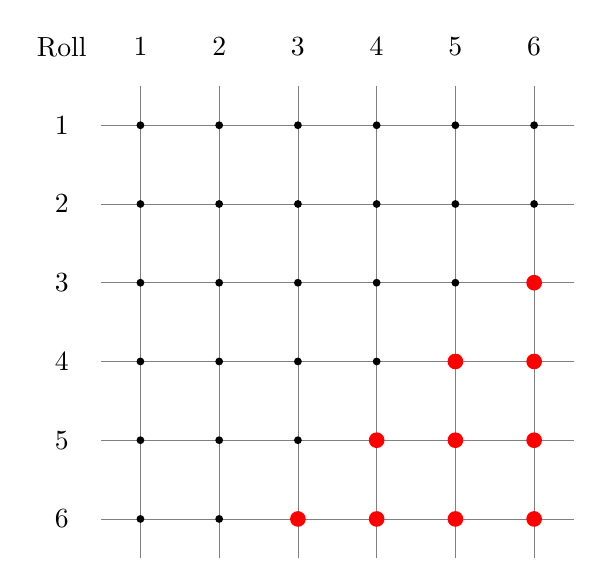
\begin{tikzpicture}[scale=1]
    % Draw grid
    \draw[step=1cm,gray,very thin] (0.5,0.5) grid (6.5,6.5);
    
    % Label rows and columns
    \foreach \x in {1,...,6} {
        \foreach \y in {1,...,6} {
            \node at (\x, 7-\y) [circle, fill, inner sep=1pt]{};
        }
        \node at (\x, 7) {\x}; % Top labels
    }
    \foreach \y in {1,...,6} {
        \node at (0, 7-\y) {\y}; % Side labels
    }
    
    % Color cells where the sum is greater than 8
    \foreach \x in {1,...,6} {
        \foreach \y in {1,...,6} {
            \pgfmathtruncatemacro{\result}{\x + \y}
            \ifnum \result>8
                \node at (\x, 7-\y) [circle, fill=red, inner sep=2pt]{};
            \fi
        }
    }
    \node at (0,7) {Roll};
\end{tikzpicture}
\end{center}

\subsubsection*{Event \(B\): First Roll is a 4}
Given the event \(B\) that the first die roll results in a 4, we focus on the fourth column of the lattice diagram, and the outcomes that contribute to \(A \cap B\) are highlighted.

% Drawing the reduced sample space for B
\begin{center}
\begin{tikzpicture}[scale=1]
    % Draw specific column for roll=4
    \draw[step=1cm,gray,very thin] (3.5,0.5) grid (4.5,6.5);
    
    % Label column and rows
    \foreach \y in {1,...,6} {
        \node at (4, 7-\y) [circle, fill, inner sep=1pt]{};
        \node at (0, 7-\y) {\y}; % Side labels
    }
    
    % Color cells where the sum is greater than 8 with the first roll = 4
    \foreach \y in {1,...,6} {
        \pgfmathtruncatemacro{\result}{4 + \y}
        \ifnum \result>8
            \node at (4, 7-\y) [circle, fill=red, inner sep=2pt]{};
        \fi
    }
    \node at (0,7) {Roll};
    \node at (4,7) {4}; % Label for the first roll
\end{tikzpicture}
\end{center}

\subsubsection*{Conditional Probability \(P(A \mid B)\)}
With \(B\) set as the first roll being 4, \(A \cap B\) involves outcomes (4,5) and (4,6), making \(P(A \cap B) = \frac{2}{36} = \frac{1}{18}\), and \(P(B) = \frac{6}{36} = \frac{1}{6}\).

Hence, the conditional probability is calculated as:
\[
P(A \mid B) = \frac{P(A \cap B)}{P(B)} = \frac{\frac{1}{18}}{\frac{1}{6}} = \frac{1}{3}.
\]
\begin{remark}
    This result is equivalent to $\frac{2}{6}=\frac{1}{3}$ in the subspace, we just use the measurement from the original sample space for clarity.
    So both explainations are acceptable, while the other one is more understandable when you cannot show the subspace.
\end{remark}
\end{example}

With this example, I believe that you must know how conditional probability is all about. However, this is only a very special case. 
You may have noticed that for rolling a fair dice, we have equal possibility to get 1-6 in each roll. In the real life, most events have different probabilities. Let's see another example of unfaired dice.
But to solve this problem, we need to use an important conclusion of conditional probability.
\begin{corollary}\label{intersectascond}
    By multiplying $P(F)$ to \( P(E \mid F) = \frac{P(EF)}{P(F)} \), we find that 
    \begin{equation}\label{intasprob}
        P(EF) = P(E \mid F)P(F)
    \end{equation}
\end{corollary}
\begin{example}\label{unfair_dice}
    An unfair four-sided die (numbered 1 to 4) is rolled twice. The biases for the die are:
    \begin{itemize}
        \item \( P(1) = 0.1 \)
        \item \( P(2) = 0.2 \)
        \item \( P(3) = 0.3 \)
        \item \( P(4) = 0.4 \)
    \end{itemize}
    We are tasked with calculating:
    \begin{enumerate}
        \item The conditional probability that the sum of the two rolls is 4, given that the first roll is a 2.
        \item The conditional probability that the first roll is a 2, given that the sum of the two rolls is 4.
    \end{enumerate}
\end{example}
\begin{solution}
    Define the events:
    \begin{itemize}
        \item \( A \): The sum of the two rolls is 4.
        \item \( B \): The first roll is a 2.
    \end{itemize}
    We can draw a tree diagram to show all possible results with possibility of each branch.
    \begin{center}
        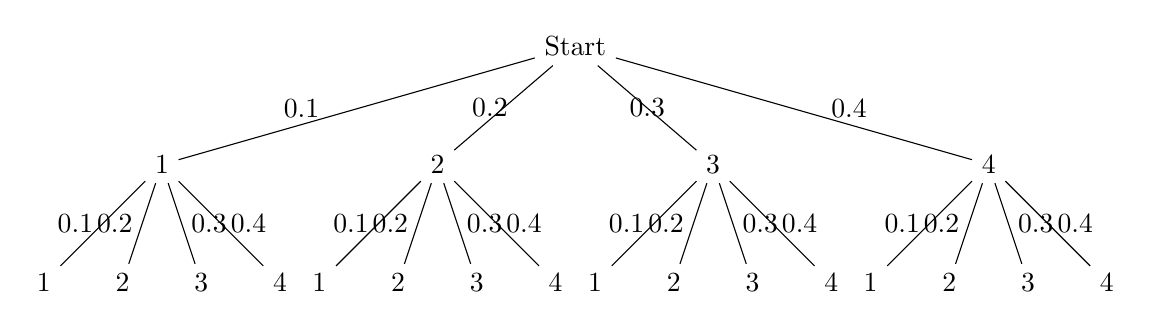
\begin{tikzpicture}[scale=1, every node/.style={align=center}, level distance=1.5cm,
          level 1/.style={sibling distance=3.5cm},
          level 2/.style={sibling distance=1cm}]
            % Level 1
            \node {Start}
                child {node {1}
                    child {node {1} edge from parent node[left] {0.1}}
                    child {node {2} edge from parent node[left] {0.2}}
                    child {node {3} edge from parent node[right] {0.3}}
                    child {node {4} edge from parent node[right] {0.4}}
                    edge from parent node[left, xshift=-10] {0.1}
                }
                child {node {2}
                    child {node {1} edge from parent node[left] {0.1}}
                    child {node {2} edge from parent node[left] {0.2}}
                    child {node {3} edge from parent node[right] {0.3}}
                    child {node {4} edge from parent node[right] {0.4}}
                    edge from parent node[left, xshift=5] {0.2}
                }
                child {node {3}
                    child {node {1} edge from parent node[left] {0.1}}
                    child {node {2} edge from parent node[left] {0.2}}
                    child {node {3} edge from parent node[right] {0.3}}
                    child {node {4} edge from parent node[right] {0.4}}
                    edge from parent node[left, xshift=10] {0.3}
                }
                child {node {4}
                    child {node {1} edge from parent node[left] {0.1}}
                    child {node {2} edge from parent node[left] {0.2}}
                    child {node {3} edge from parent node[right] {0.3}}
                    child {node {4} edge from parent node[right] {0.4}}
                    edge from parent node[right, xshift=10] {0.4}
                };
        \end{tikzpicture}
        \end{center}
    \subsubsection*{1. \( P(A \mid B) \)}
    The event \( B \) fixes the first roll at 2. For \( A \) to occur with \( B \), the second roll must be 2 (i.e., \( 2 + 2 = 4 \)).
    \[ P(A \mid B) = P(\text{Second roll is 2}) = P(2) = 0.2 \]
    This could also easily be examined from the graph the 2-2 is the only branch among the four possible cases under 2 in the first roll, so we have $P(A \mid B) = \frac{0.2\times 0.2}{0.2}=0.2$.
    \begin{remark}
        We get $P(A \mid B) = \frac{0.2\times 0.2}{0.2}=0.2$ by using the corollary to the numerator, which is the probability of getting a two twice. 
        By the corollary, it can be expressed as the product of the probability we get 2 in the second trial given that 2 is ontained in the first attempt, and $P(2)$.
        It is obvious that the condition does not work here, because we always have the same chance of getting a 2. Thus we have $0.2^2$ as the numerator of $P(A \mid B)$.
    \end{remark}
    \subsubsection*{2. \( P(B \mid A) \)}
    The event \( A \) (sum is 4) can occur through the following combinations:
    \begin{itemize}
        \item \( (1, 3) \) and \( (3, 1) \)
        \item \( (2, 2) \)
    \end{itemize}
    
    Calculate \( P(A) \):
    \[ P(A) = P(1, 3) + P(3, 1) + P(2, 2) = 0.1 \cdot 0.3 + 0.3 \cdot 0.1 + 0.2 \cdot 0.2 = 0.03 + 0.03 + 0.04 = 0.1 \]
    \begin{remark}
        Note that: 
        \begin{itemize}
            \item We use Eq \ref{intasprob} here, since for some event $E,F$, $P(E\cap F) = P(E \mid F)P(F)$.
            We get the probability of each branch by using the RHS of the equation using the probability on the edge of the tree 
            diagram. E.g., we have 3 for the second roll and 1 in the first roll, then we have $0.3\times 0.1 = 0.03$ chance for the coresponding result.
            \item The weight on the tree graph in every layer are treated as conditional probability, and 0.3 is the probability of a three given that the first roll gives 1
            \item Also notice that all branches are disjoint, so we use additibity axiom here to 
            sum up the probability.
        \end{itemize}

    \end{remark}
    Now, \( P(B \mid A) \):
    \[ P(B \mid A) = \frac{P(B \cap A)}{P(A)} = \frac{P(2, 2)}{P(A)} = \frac{0.04}{0.1} = 0.4 \]
    
 From this example we see that despite that we have different probability for each branch of events, what we are doing to find conditional probability is still the same:
 subsetting the sample space and locate our target cases in that subspace.
\end{solution}

We wrap up the use of lattice diagram and tree diagram here.
    \subsubsection*{Lattice Diagram}
    Lattice diagrams are particularly useful for representing all possible outcomes in a sequence of events where outcomes are straightforward and often \textbf{uniformly distributed}, such as 
    flipping coins or rolling dice. They are excellent for visualizing permutations, combinations, and the structure of outcomes in multi-stage experiments. A lattice diagram efficiently showcases how different
    paths can lead to various results, making it ideal for illustrating scenarios with equal probabilities or for modeling situations like financial derivatives pricing, where the path dependencies of 
    options or other financial instruments are important.
    \subsubsection*{Tree Diagram}
    Tree diagrams, on the other hand, excel in situations where outcomes have different probabilities(i.e., \textbf{not uniformly distributed} ) or the process is inherently hierarchical. They are invaluable for breaking down complex probability problems into 
    manageable parts, especially in Bayesian statistics where updates to probability estimates are made as new information becomes available. Tree diagrams allow for the visualization of conditional probabilities 
    and sequential decision processes, making them perfect for scenarios where events are dependent on previous outcomes, such as sequential games, Bayesian inference, or decision analysis.

    But of course, we will not always use diagram for problem-solving, since you can imagine how complex the diagram could be when the scale of the problem increases. Fundamentally,
    we still need to obtain the result by analyzing the chain of events and their relations with the given conditions in different contexts.

    Here are some more interesting examples.

    \begin{example}
        Celine is undecided whether to take a French course or a chemistry course. She estimates that her probability of receiving an A grade would be \(\frac{1}{2}\) in a French course and \(\frac{2}{3}\) in a chemistry course. If Celine decides to base her decision on the flip of a fair coin, what is the probability that she gets an A in chemistry?
        \end{example}
        
        \begin{solution}
        Let \( C \) be the event that Celine takes the chemistry course and \( A \) be the event that she receives an A in whatever course she takes. The decision to take chemistry is based on the flip of a fair coin, thus \( P(C) = \frac{1}{2} \).
        
        Given \( C \) (the event of taking chemistry), the probability of \( A \) (receiving an A) in chemistry is \( P(A \mid C) = \frac{2}{3} \). Therefore, the probability that Celine takes chemistry and gets an A can be calculated using the rule of multiplication for probabilities:
        
        \[
        P(CA) = P(C)P(A \mid C) = \left(\frac{1}{2}\right)\left(\frac{2}{3}\right) = \frac{1}{3}.
        \]
        
        Thus, the probability that Celine gets an A in chemistry, given that her decision is based on a coin flip, is \(\frac{1}{3}\).
        \end{solution}
        \begin{remark}
        Some people may wonder why we are calculating probability of intersection instead of conditional probability here. Because semantically, the probability of getting A in chemistry
        \textbf{given that} we get head/tail of the coin seems equivalent to the probability of getting A in chemistry, \textbf{and} we get head/tail of the coin. The answer if completely NO.
        Because when we gauge the conditional probability, condition(s) matters. Will the result of flipping the coin affact the chance of getting A in chemistry? Of course no, so we are not finding
        a conditional probability. We will discuss this further in independence of events. This is a vivid example that demonstrates the difference of sumbolic language and natural language. The former
        outperforms in terms of accuracy but less understandable for human, while natural language is more understandable but in many cases, bring a lot of bias.
        \end{remark}

        \begin{example}
            Suppose that an urn contains 8 red balls and 4 white balls. We draw 2 balls from the urn without replacement.
            
            \textbf{(a)} If we assume that at each draw, each ball in the urn is equally likely to be chosen, what is the probability that both balls drawn are red?
            
            \textbf{(b)} Now suppose that the balls have different weights, with each red ball having weight \(r\) and each white ball having weight \(w\). Suppose that the probability that a given ball in the urn is the next one selected is its weight divided by the sum of the weights of all balls currently in the urn. Now what is the probability that both balls are red?
            \end{example}
            
            \begin{solution}
            \textbf{(a)} Let \( R_1 \) and \( R_2 \) denote, respectively, the events that the first and second balls drawn are red. Given that the first ball selected is red, there are 7 remaining red balls and 4 white balls, so \( P(R_2|R_1) = \frac{7}{11} \). As \( P(R_1) \) is clearly \(\frac{8}{12}\), the desired probability is calculated as:
            \[
            P(R_1 R_2) = P(R_1)P(R_2|R_1) = \left(\frac{2}{3}\right)\left(\frac{7}{11}\right) = \frac{14}{33}.
            \]
            
            \textbf{(b)} For this part, we again let \( R_i \) be the event that the \(i\)-th ball chosen is red and use:
            \[
            P(R_1 R_2) = P(R_1)P(R_2|R_1)
            \]
            Now, number the red balls, and let \( B_i, i = 1, \ldots, 8 \) be the event that the first ball drawn is red ball number \( i \). Then:
            \[
            P(R_1) = P\left(\bigcup_{i=1}^8 B_i\right) = \sum_{i=1}^8 P(B_i) = \frac{8r}{8r + 4w}
            \]
            Moreover, given that the first ball is red, the urn then contains 7 red and 4 white balls. Thus, by a similar argument:
            \[
            P(R_2|R_1) = \frac{7r}{7r + 4w}
            \]
            Hence, the probability that both balls are red is:
            \[
            P(R_1 R_2) = \frac{8r}{8r + 4w} \times \frac{7r}{7r + 4w} = \frac{8r \times 7r}{(8r + 4w)(7r + 4w)}
            \]
            \end{solution}
    
        Now let's move further onto the generalization of corollary \ref{intersectascond}, known as The multiplication rule of probability.
        Multiplication rule is used to calculate the probability of an event after a chain of event.
        In fact, we are using the previous definition multiple times here.
        
        \begin{theorem}[Multiplication Rule]
            If \(E_1, E_2, \ldots, E_n\) are events, then the probability of all these events occurring in sequence is given by:
            \[
            P(E_1 E_2 \cdots E_n) = P(E_1) P(E_2 \mid E_1) P(E_3 \mid E_1 E_2) \cdots P(E_n \mid E_1 E_2 \cdots E_{n-1})
            \]
            \end{theorem}
            
            \begin{proof}
            We prove the theorem by induction on the number of events \(n\).
            
            \textbf{Base case} (\(n = 2\)): For two events \(E_1\) and \(E_2\), the multiplication rule reduces to:
            \[
            P(E_1 E_2) = P(E_1) P(E_2 \mid E_1),
            \]
            which is the definition of the conditional probability of \(E_2\) given \(E_1\).
            
            \textbf{Inductive step}: Assume that the theorem holds for \(n-1\) events. That is, we assume:
            \[
            P(E_1 E_2 \cdots E_{n-1}) = P(E_1) P(E_2 \mid E_1) \cdots P(E_{n-1} \mid E_1 \cdots E_{n-2}).
            \]
            We need to prove that the rule holds for \(n\) events. By the definition of conditional probability, we have:
            \[
            P(E_1 E_2 \cdots E_n) = P(E_1 E_2 \cdots E_{n-1}) P(E_n \mid E_1 E_2 \cdots E_{n-1}).
            \]
            Applying the induction hypothesis, we substitute for \(P(E_1 E_2 \cdots E_{n-1})\):
            \[
            P(E_1 E_2 \cdots E_n) = \left(P(E_1) P(E_2 \mid E_1) \cdots P(E_{n-1} \mid E_1 \cdots E_{n-2})\right) P(E_n \mid E_1 \cdots E_{n-1}),
            \]
            which confirms the theorem for \(n\) events.
            
            Thus, by the principle of mathematical induction, the multiplication rule holds for any number of events.
        \end{proof}
        \begin{remark}
            Actually, we have a more decent way to prove it, which works like chain rule in differentiation.To prove the multiplication rule, just apply the definition of conditional probability
            to its right-hand side, giving
            \[P(E_1)\frac{P(E_1E_2)}{P(E_1)}\frac{P(E_1E_2E_3)}{P(E_1E_2)}\cdots\frac{P(E_1E_2\cdots E_n)}{P(E_1E_2\cdots E_{n-1})}=P(E_1E_2\cdots E_n).\]
        \end{remark}

        \begin{example}
            An ordinary deck of 52 playing cards is randomly divided into 4 piles of 13 cards each. Compute the probability that each pile has exactly 1 ace.
            \begin{solution}
            Define events \(E_i\), \(i = 1, 2, 3, 4\), as follows:
            \begin{itemize}
                \item \(E_1 = \{\text{the ace of spades is in any one of the piles}\}\)
                \item \(E_2 = \{\text{the ace of spades and the ace of hearts are in different piles}\}\)
                \item \(E_3 = \{\text{the aces of spades, hearts, and diamonds are all in different piles}\}\)
                \item \(E_4 = \{\text{all 4 aces are in different piles}\}\)
            \end{itemize}
            
            The desired probability is \(P(E_1 E_2 E_3 E_4)\), and by the multiplication rule,
            \[
            P(E_1 E_2 E_3 E_4) = P(E_1) P(E_2 \mid E_1) P(E_3 \mid E_1 E_2) P(E_4 \mid E_1 E_2 E_3)
            \]
            
            Now, \(P(E_1) = 1\) since \(E_1\) is the sample space \(S\). To determine \(P(E_2 \mid E_1)\), consider the pile that contains the ace of spades. Because its remaining 12 cards are equally likely to be any 12 of the remaining 51 cards, the probability that the ace of hearts is among them is \(12/51\), giving that
            \[
            P(E_2 \mid E_1) = 1 - \frac{12}{51} = \frac{39}{51}
            \]
            
            Also, given that the ace of spades and ace of hearts are in different piles, it follows that the set of the remaining 24 cards of these two piles is equally likely to be any set of 24 of the remaining 50 cards. As the probability that the ace of diamonds is one of these 24 is \(24/50\), we see that
            \[
            P(E_3 \mid E_1 E_2) = 1 - \frac{24}{50} = \frac{26}{50}
            \]
            
            Because the same logic as used in the preceding yields that
            \[
            P(E_4 \mid E_1 E_2 E_3) = 1 - \frac{36}{49} = \frac{13}{49}
            \]
            
            the probability that each pile has exactly 1 ace is
            \[
            P(E_1 E_2 E_3 E_4) = \frac{39}{51} \cdot \frac{26}{50} \cdot \frac{13}{49} \approx 0.105
            \]
            
            That is, there is approximately a 10.5 percent chance that each pile will contain an ace. (Problem 13 gives another way of using the multiplication rule to solve this problem.)
            \end{solution}
            \end{example}
	
	\subsection{Exercises}
	
	
\section{Bayes's Theorem}
\subsection{Bayes's Theorem and Bayesian Thinking}
        We can do more with conditional probability. Now consider event $E$ and $F$. Regardless of what kind of events they are, we always have 
        \[E = EF \cup EF^c.\]
        This makes sense not only from set theory's conclusion but also in terms of practicality. Because for any two events, assuming one of them will happen, then the other one could either happen or not happen.
        We know that \( EF \tx{ and } EF^c\) are mutually exclusive, so by additivity axiom, we have 
        \begin{equation}
        	\begin{aligned}
        		P(E)& =P(EF) + P(EF^c) \\
        		&=P(E|F)P(F) + P(E|F^c)P(F^c) \\
        		&=P(E|F)P(F) + P(E|F^c)\bigl[1 - P(F)\bigr].
        	\end{aligned}
        \end{equation}
        This can be interpreted as: the probability of the event E is measured by the weighted average of of the possibility that F happens and not happens. This formula enables us to get the probability of an event by conditioning the probability of some other events and its complement.
        This is very important for us, since some times we cannot get the probability of a certain event easily. The following example shows its advantage in finding conditional probability (in a reversed order).
        \begin{example}
        	An insurance company believes that people can be divided into two classes: those who are accident prone and those who are not. The company's statistics show that an accident-prone person will have an accident at some time within a fixed 1-year period with probability .4, whereas this probability decreases to .2 for a person who is not accident prone. If we assume that 30 percent of the population is accident prone, what is the probability that a new policyholder will have an accident within a year of purchasing a policy?
        	
        	\begin{solution}
        		We shall obtain the desired probability by first conditioning upon whether or not the policyholder is accident prone. Let \(A_1\) denote the event that the policyholder will have an accident within a year of purchasing the policy, and let \(A\) denote the event that the policyholder is accident prone. Hence, the desired probability is given by
        		\[
        		P(A_1) = P(A_1 \mid A)P(A) + P(A_1 \mid A^c)P(A^c) = (0.4)(0.3) + (0.2)(0.7) = 0.26
        		\]
        	\end{solution}
        \end{example}
        Note that in the previous example, we used the probability of $A_1$ given $A$ or $A^c$. The next example shows how we can get the probability of $A$ given $A_1$. 
        \begin{example}
        	Suppose that a new policyholder has an accident within a year of purchasing a policy. What is the probability that he or she is accident prone?
        	
        	\begin{solution}
        		The desired probability is
        		\[
        		P(A \mid A_1) = \frac{P(A \cap A_1)}{P(A_1)} = \frac{P(A_1 \mid A)P(A)}{P(A_1)} = \frac{(0.3)(0.4)}{0.26} = \frac{6}{13}
        		\]
        	\end{solution}
        \end{example}
        
       With this example, we have determined that knowing the probability of an event $E$ (in this case, we can obtain its complement $E^c$ using the complement rule such that $P(E^c) = 1 - P(E)$), given another event $F$ and its complement $F^c$, enables us to calculate the probability of $F$ given $E$.
       
       This is known as Bayes's Theorem. The interesting part of the theorem lies not only in terms of algebra or practical significance, but it also illustrates a thinking pattern.
       \begin{theorem}[Bayes's Theorem]
       	 Given two events $A$ and $B$, with $P(B) > 0$, Bayes' theorem describes the probability of event $A$ given that event $B$ has occurred, and is formally defined as:
       	\[
       	P(A|B) = \frac{P(B|A)P(A)}{P(B)}
       	\]
       	where:
       	\begin{itemize}
       		\item $P(A|B)$ is the \textit{posterior probability} of event $A$ occurring given the occurrence of event $B$.
       		\item $P(B|A)$ is the \textit{likelihood}, which is the probability of observing event $B$ given that event $A$ has occurred.
       		\item $P(A)$ is the \textit{prior probability} of event $A$ occurring.
       		\item $P(B)$ is the \textit{marginal probability} of event $B$, which can also be calculated using the law of total probability if the complete set of outcomes related to $A$ is known:
       		\[
       		P(B) = \sum_{i} P(B|A_i)P(A_i)
       		\]
       	\end{itemize}
       \end{theorem}
       The Bayes's Formula is extremely concise and easy to understand, however profound philosophical and cognitive significance are combined into this expression. 
       
       Bayes's formula models the way human make judgment, of course, in a wise way. For each term of the formula, we have given an definition, which we need to figure out.
       \begin{itemize}
       	\item The prior probability is the existing belief in a certain event.
       	\item The likelihood is an factor that helps people make further judgment, which means the possibility of something else to happen under some given facts(in someone's mind, but may not a 100\% true fact).
       	\item The marginal probability refers to the possibility of the other related event. 
       	\item Posterior Probability refers to the new possibility given some other event(s) that fix/update the prior probability to a reasonable level.
       \end{itemize}
       If I tell you, this is exactly how human-beings , not just as an individual, but a civilization, learn, you may confuse that these seem very elusive and abstract, but we can clarify this by using one example.
       
       Consider asking the question that "Is the earth flat or a sphere" to someone randomly picked from somewhere in the world, almost everyone will say yes, out of common sense. But clearly people do not always think so.
       In the past, or more specifically, before human-beings grasp the way of examine and measuring the nature, most people believe that we live on a flat land. However, with the advance of sailing technique, thrive of colonialism, and a cascade of geographical discovery, some people slightly change their mind, finding some tiny possibility that we live on a sphere. Only until the first global circling sail is done, that the earth is a sphere becomes acceptable to more and more people and finally become a common sense.
       
       In this example, the prior probability of the event that the earth of is flat decreases, while the possibility of the contradictory event that the earth of sphere increases. We can analyze the numerator and denominator of the formula, and we will find that  $P(A)$ approaches to 0 and
       $P(B)$ approaches to 1. Eventually, this makes the probability that earth is flat given all new known facts(observation from $B$) to almost 0. This is exactly how we learn new things.
       
       Though we know the interesting example, we still cannot prove it. We have shown how this makes sense previously, but only one thing is different here, since we consider that there could be any amount $i$ out comes for $A$, while previously we used the base case where $A$ is a binary event, meaning it is only considered happen or not happen.
       
       To work this problem out, we first introduces the law of total probability.
       \begin{theorem}[Law of Total Probability]
       	Let \(B_1, B_2, \ldots, B_n\) be a finite or countably infinite partition of the sample space \(S\), such that \(B_i \cap B_j = \emptyset\) for all \(i \neq j\) and \(\bigcup_{i=1}^n B_i = S\), with \(P(B_i) > 0\) for all \(i\). For any event \(A\) in \(S\),
       	\[
       	P(A) = \sum_{i=1}^n P(A \mid B_i) P(B_i).
       	\]
       \end{theorem}
       \begin{proof}
       	Consider the event \(A\) and the partition \(B_1, B_2, \ldots, B_n\) of the sample space \(S\). Since these sets are mutually exclusive and collectively exhaustive,
       	\[
       	A = A \cap S = A \cap \left( \bigcup_{i=1}^n B_i \right) = \bigcup_{i=1}^n (A \cap B_i) \tx{ (Set Distributive Law)}.
       	\]
       	Because the sets \(A \cap B_i\) are mutually exclusive,
       	\[
       	P(A) = P\left( \bigcup_{i=1}^n (A \cap B_i) \right) = \sum_{i=1}^n P(A \cap B_i).
       	\]
       	Using the definition of conditional probability,
       	\[
       	P(A \cap B_i) = P(A \mid B_i) P(B_i).
       	\]
       	Thus,
       	\[
       	P(A) = \sum_{i=1}^n P(A \mid B_i) P(B_i),
       	\]
       	which is the statement of the law of total probability.
       \end{proof}
       \begin{remark}
       	You may also prove this by induction with $n=2$ as a base case using the conclusion of the beginning of the section.
       \end{remark}
       Now we can proceed to prove Bayes's Theorem.
       \begin{proof}[Proof of Bayes's Theorem]
       	Assume \( B_1, B_2, \ldots, B_n \) is a partition of the sample space, and \( A \) is any event in the sample space. According to the law of total probability, we have:
       	\[
       	P(A) = \sum_{i=1}^n P(A \cap B_i)
       	\]
       	Using the definition of conditional probability, we express \( P(A \cap B_i) \) as:
       	\[
       	P(A \cap B_i) = P(A | B_i)P(B_i)
       	\]
       	Substituting this back into the law of total probability, we obtain:
       	\[
       	P(A) = \sum_{i=1}^n P(A | B_i)P(B_i)
       	\]
       	Now, consider the conditional probability \( P(B_j | A) \) for some \( j \). By definition, it is:
       	\[
       	P(B_j | A) = \frac{P(A \cap B_j)}{P(A)}
       	\]
       	Substituting \( P(A \cap B_j) = P(A | B_j)P(B_j) \) into the equation, we get:
       	\[
       	P(B_j | A) = \frac{P(A | B_j)P(B_j)}{P(A)}
       	\]
       	Since \( P(A) \) can be expanded using the law of total probability, it becomes:
       	\[
       	P(B_j | A) = \frac{P(A | B_j)P(B_j)}{\sum_{i=1}^n P(A | B_i)P(B_i)}
       	\]
       	This equation is Bayes' Theorem for the case where the partition \( \{B_i\} \) consists of \( n \) events. For the simpler case with only one \( B \) and its complement \( B^c \), Bayes' Theorem simplifies to:
       	\[
       	P(B | A) = \frac{P(A | B)P(B)}{P(A | B)P(B) + P(A | B^c)P(B^c)}
       	\]
       \end{proof}
       Here are some typical problems.
       \begin{example}
       	At a certain stage of a criminal investigation, the inspector in charge is \(60\%\) convinced of the guilt of a certain suspect. Suppose, however, that a new piece of evidence which shows that the criminal has a certain characteristic (such as left-handedness, baldness, or brown hair) is uncovered. If \(20\%\) of the population possesses this characteristic, how certain of the guilt of the suspect should the inspector now be if it turns out that the suspect has the characteristic?
       	\begin{solution}
       		Let \( G \) denote the event that the suspect is guilty and \( C \) the event that he possesses the characteristic of the criminal. We use Bayes' theorem to update our belief about \( G \) given \( C \):
       		\[
       		P(G \mid C) = \frac{P(G \cap C)}{P(C)}
       		\]
       		Applying the law of total probability to the denominator,
       		\[
       		P(C) = P(C \mid G)P(G) + P(C \mid G^c)P(G^c)
       		\]
       		Given that \( P(G) = 0.60 \) and \( P(G^c) = 0.40 \) (since the suspect being not guilty is the complement of the suspect being guilty), and assuming \( P(C \mid G) = 1.0 \) (if the suspect is guilty, he definitely has the characteristic) and \( P(C \mid G^c) = 0.20 \) (the probability that a non-guilty person has the characteristic),
       		\[
       		P(C) = (1.0)(0.60) + (0.20)(0.40) = 0.60 + 0.08 = 0.68
       		\]
       		Thus,
       		\[
       		P(G \mid C) = \frac{P(C \mid G)P(G)}{P(C)} = \frac{(1.0)(0.60)}{0.68} \approx 0.882
       		\]
       		This indicates that, given the suspect has the characteristic, the inspector should now be approximately \(88.2\%\) certain of the suspect's guilt.
       	\end{solution}
       \end{example}
       
       \begin{example}
       	Suppose that we have 3 cards that are identical in form, except that both sides of the first card are colored red, both sides of the second card are colored black, and one side of the third card is colored red and the other side black. The 3 cards are mixed up in a hat, and 1 card is randomly selected and put down on the ground. If the upper side of the chosen card is colored red, what is the probability that the other side is also colored red?
       
       \begin{solution}
       	Let \( RR \), \( BB \), and \( RB \) denote, respectively, the events that the chosen card is all red, all black, or the red--black card. Also, let \( R \) be the event that the upturned side of the chosen card is red. Then, the desired probability is obtained by
       	\[
       	P(R_B \mid R) = \frac{P(R_B \cap R)}{P(R)}
       	\]
       	where \( R_B \) is the event that the bottom side is red. We compute \( P(R) \) using the law of total probability:
       	
       	\begin{align*}
       		P(R) &= P(R \mid RR)P(RR) + P(R \mid RB)P(RB) + P(R \mid BB)P(BB)\\
       			& = \left(\frac{1}{2}\right)\left(\frac{1}{3}\right) + \left(\frac{1}{2}\right)\left(\frac{1}{3}\right) + 0\left(\frac{1}{3}\right) = \frac{1}{3}
       	\end{align*}
       	
       	and
       	\[
       	P(R_B \cap R) = P(R \mid RR)P(RR) = \left(\frac{1}{2}\right)\left(\frac{1}{3}\right) = \frac{1}{6}
       	\]
       	Thus,
       	\[
       	P(R_B \mid R) = \frac{\frac{1}{6}}{\frac{1}{3}} = \frac{1}{2}
       	\]
       	Hence, the answer is \(\frac{1}{3}\). Some students guess \(\frac{1}{2}\) as the answer by incorrectly reasoning that given that a red side appears, there are two equally likely possibilities: that the card is the all-red card or the red--black card. Their mistake, however, is in assuming that these two possibilities are equally likely. For, if we think of each card as consisting of two distinct sides, then we see that there are 6 equally likely outcomes of the experiment -- namely, \(R_1, R_2, B_1, B_2, R_3, B_3\) -- where the outcome is \(R_1\) if the first side of the all-red card is turned face up, \(R_2\) if the second side of the all-red card is turned face up, \(R_3\) if the red side of the red--black card is turned face up, and so on. Since the other side of the upturned red side will be black only if the outcome is \(R_3\), we see that the desired probability is the conditional probability of \(R_3\) given that either \(R_1\) or \(R_2\) or \(R_3\) occurred, which obviously equals \(\frac{1}{3}\).
       \end{solution}
    	\end{example}
    	
    	Sometimes we cannot solve the problem with Bayes's Theorem, and we have to calculate the probability for specific cases by parameter estimation. Here is an example.
    	
    	\begin{example}
    		A new couple, known to have two children, has just moved into town. Suppose that the mother is encountered walking with one of her children. If this child is a girl, what is the probability that both children are girls?
    		\begin{solution}
    			Let us start by defining the following events:
    			\begin{itemize}
    				\item \( G_1 \): the first (that is, the oldest) child is a girl.
    				\item \( G_2 \): the second child is a girl.
    				\item \( G \): the child seen with the mother is a girl.
    			\end{itemize}
    			Also, let \( B_1, B_2, \) and \( B \) denote similar events, except that ``girl'' is replaced by ``boy.'' Now, the desired probability is \( P(G_1 G_2 \mid G) \), which can be expressed as follows:
    			\[
    			P(G_1 G_2 \mid G) = \frac{P(G_1 G_2 \cap G)}{P(G)}
    			\]
    			where \( P(G) \) can be calculated using the law of total probability:
    			\[
    			P(G) = P(G \mid G_1 G_2) P(G_1 G_2) + P(G \mid G_1 B_2) P(G_1 B_2) + P(G \mid B_1 G_2) P(B_1 G_2) + P(G \mid B_1 B_2) P(B_1 B_2)
    			\]
    			Given that \( P(G \mid G_1 G_2) = 1 \) and \( P(G \mid G_1 B_2) = 0.5 \) and \( P(G \mid B_1 G_2) = 0.5 \) and \( P(G \mid B_1 B_2) = 0 \), and assuming that all four gender combinations are equally likely (\( \frac{1}{4} \) each),
    			\[
    			P(G) = 1 \cdot \frac{1}{4} + \frac{1}{2} \cdot \frac{1}{4} + \frac{1}{2} \cdot \frac{1}{4} + 0 \cdot \frac{1}{4} = \frac{1}{2}
    			\]
    			Now, \( P(G_1 G_2) \) is simply the probability of having two girls, which is \( \frac{1}{4} \), so
    			\[
    			P(G_1 G_2 \cap G) = P(G_1 G_2) = \frac{1}{4}
    			\]
    			Therefore,
    			\[
    			P(G_1 G_2 \mid G) = \frac{\frac{1}{4}}{\frac{1}{2}} = \frac{1}{2}
    			\]
    			Thus, if the child seen is a girl, the probability that both children are girls is \( \frac{1}{2} \).
    		\end{solution}
    	\end{example}
    	
    	\subsection{Exercises}
    	
\section{Independence of Events}

\subsection{Definition of Independence}
previously, we defined the conditional probability of some event $E$ given $F$
by \[P(E\mid F)= \frac{P(EF)}{P(F)}.\]

You may recall that, in some examples earlier, we find $P(E\mid F) = P(E)$,
and we have $P(E\mid F)=P(E) \iff P(EF) = P(E) \times P(F)$. In this case, we claim that 
$E$ is independent of $F$.
\begin{definition}
    Two events E and F are said to be independent if and only if 
    \begin{equation}
        P(E\mid F)=P(E) \iff P(EF) = P(E) \times P(F)
    \end{equation}
\end{definition}
Here's a basic example.
\begin{example}
    Suppose that we toss two fair dice. Consider the following events:
\begin{itemize}
    \item \(E_1\): The event that the sum of the dice is 6.
    \item \(F\): The event that the first die equals 4.
\end{itemize}
We are interested in determining whether these two events are independent.
\begin{solution}
    First, calculate \(P(E_1)\) and \(P(F)\), and then \(P(E_1 \cap F)\) to check for independence:
\begin{itemize}
    \item The probability that the sum of the dice equals 6, \(P(E_1)\), can happen through the combinations \((1,5), (2,4), (3,3), (4,2), (5,1)\). Thus,
    \[
    P(E_1) = \frac{5}{36}
    \]
    because there are 5 favorable outcomes out of 36 possible outcomes when two dice are thrown.
    
    \item The probability that the first die equals 4, \(P(F)\), is simply,
    \[
    P(F) = \frac{1}{6}
    \]
    since one out of six faces of a die shows 4.

    \item The probability of both \(E_1\) and \(F\) occurring, \(P(E_1 \cap F)\), happens only if the first die is 4 and the second die is 2 (to make the sum 6). Thus,
    \[
    P(E_1 \cap F) = \frac{1}{36}
    \]
    because there is only one favorable outcome for this combination under the condition that two dice are thrown.
\end{itemize}

Now, to check for independence, we examine if \(P(E_1 \cap F) = P(E_1)P(F)\):
\[
P(E_1)P(F) = \left(\frac{5}{36}\right)\left(\frac{1}{6}\right) = \frac{5}{216}
\]
Clearly, \(\frac{1}{36} \neq \frac{5}{216}\), indicating that \(E_1\) and \(F\) are \textbf{not independent}.
\end{solution}
\end{example}
Another fact about independent event is that if two events are independent to each other, then they are also independent of each other's complement event.
\begin{proposition}
    If \(E\) and \(F\) are independent, then so are \(E\) and \(F^c\).
    \end{proposition}
    \begin{proof}
        Assume that \(E\) and \(F\) are independent. Since \(E\) can be expressed as the union of disjoint events \(EF\) and \(EF^c\), we write
        \[
        P(E) = P(EF) + P(EF^c).
        \]
        Using the independence of \(E\) and \(F\), we have
        \[
        P(EF) = P(E)P(F).
        \]
        Thus, the probability of \(E\) can be rewritten using the complement rule as
        \[
        P(E) = P(E)P(F) + P(EF^c).
        \]
        Rearranging terms gives
        \[
        P(EF^c) = P(E) - P(E)P(F) = P(E)(1 - P(F)) = P(E)P(F^c).
        \]
        Hence, \(P(EF^c) = P(E)P(F^c)\) shows that \(E\) and \(F^c\) are independent.
        \end{proof}
    
    \subsection{Multiple Independence}
    We have discussed the base case of independence between two events, how it is like for more events? Here is an example.
    \begin{example}
        Two fair dice are thrown. Let \( E \) denote the event that the sum of the dice is 7. Let \( F \) denote the event that the first die equals 4 and \( G \) denote the event that the second die equals 3. From earlier discussions, we know that \( E \) is independent of \( F \), and the same reasoning shows that \( E \) is also independent of \( G \). However, we find that \( E \) is not independent of the joint event \( FG \) because \( P(E \mid FG) = 1 \).
Given:
\begin{itemize}
    \item \( E \): Sum of two dice is 7.
    \item \( F \): First die is 4.
    \item \( G \): Second die is 3.
\end{itemize}
\begin{solution}
    \textbf{Independence Analysis:}
\begin{itemize}
    \item \( E \) and \( F \) are independent:
    \[
    P(E \cap F) = P(E)P(F) \implies \frac{1}{36} = \left(\frac{1}{6}\right)\left(\frac{1}{6}\right) = \frac{1}{36}
    \]
    \item \( E \) and \( G \) are independent:
    \[
    P(E \cap G) = P(E)P(G) \implies \frac{1}{36} = \left(\frac{1}{6}\right)\left(\frac{1}{6}\right) = \frac{1}{36}
    \]
    \item \( E \) and \( FG \) are not independent since:
    \[
    P(E \mid FG) = 1 \quad (\text{since if \( F \) and \( G \) occur, the sum is automatically 7})
    \]
    \[
    P(E \cap FG) = P(FG) \neq P(E)P(FG)
    \]
    Indeed, \( P(FG) = \frac{1}{36} \) and \( P(E) = \frac{1}{6} \), so:
    \[
    P(E)P(FG) = \left(\frac{1}{6}\right)\left(\frac{1}{36}\right) = \frac{1}{216} \neq \frac{1}{36}
    \]
\end{itemize}

Thus, while \( E \) is independent of both \( F \) and \( G \) individually, it is not independent of the joint event \( FG \), illustrating how independence between individual events does not necessarily extend to independence with joint events.
\end{solution}
    \end{example}
    \begin{definition}[Multiple Independence]
        Three events \(E\), \(F\), and \(G\) are said to be independent if the following conditions hold:
        \begin{align*}
        P(EFG) &= P(E)P(F)P(G), \\
        P(EF) &= P(E)P(F), \\
        P(EG) &= P(E)P(G), \\
        P(FG) &= P(F)P(G).
        \end{align*}
        \end{definition}

        Note that if $E,F$, and $G$ are independent, then $E$ will be independent of any
        event formed from $F$ and $G.$ For instance, $E$ is independent of $F\cup G$,since
        \[\begin{aligned}P[E(F\cup G)]&=P(EF\cup EG)\\&=P(EF)\:+\:P(EG)\:-\:P(EFG)\\&=P(E)P(F)\:+\:P(E)P(G)\:-\:P(E)P(FG)\\&=P(E)[P(F)\:+\:P(G)\:-\:P(FG)]\\&=P(E)P(F\:\cup\:G)\end{aligned}\]
        You may find that this notion is kind of like inclusion-exclusion, and the only difference is that
        we are not taking the case of one object into account. We can easily extend the definition of 
        independence to infinitely many events, which will be an exercise probelm.

    \begin{example}
        Consider an infinite sequence of independent trials, each resulting in a success with probability \( p \) and a failure with probability \( 1 - p \). Determine the probability that:
\begin{enumerate}
    \item[(a)] At least 1 success occurs in the first \( n \) trials.
    \item[(b)] Exactly \( k \) successes occur in the first \( n \) trials.
    \item[(c)] All trials result in successes.
\end{enumerate}
\begin{solution}
(a) Probability of at least one success in the first \( n \) trials

To find this probability, it's easiest to first compute the probability of the complementary event: no successes in the first \( n \) trials. If \( E_i \) denotes a failure on the \( i \)-th trial, by independence, the probability of no successes is:
\[
P(E_1 E_2 \ldots E_n) = P(E_1)P(E_2) \cdots P(E_n) = (1-p)^n
\]
Thus, the probability of at least one success is:
\[
P(\text{at least one success}) = 1 - P(\text{no successes}) = 1 - (1-p)^n
\]

(b) Probability of exactly \( k \) successes in the first \( n \) trials

Consider any specific sequence of \( n \) outcomes containing \( k \) successes and \( n - k \) failures. Each sequence occurs with probability \( p^k (1-p)^{n-k} \), and the number of such sequences is given by the binomial coefficient \(\binom{n}{k}\):
\[
P(\text{exactly } k \text{ successes}) = \binom{n}{k} p^k (1-p)^{n-k}
\]

(c) Probability that all trials result in successes
By part (a), the probability that the first \( n \) trials all result in success is \( p^n \). The event that all trials result in success is the intersection of the events of success on each trial, \( E_i \), over an infinite number of trials. Using the continuity property of probabilities:
\[
P(\bigcap_{i=1}^\infty E_i) = \lim_{n \to \infty} P(E_1 E_2 \ldots E_n) = \lim_{n \to \infty} p^n
\]
This limit is 0 if \( p < 1 \) and 1 if \( p = 1 \), reflecting that only if success is certain on every trial (i.e., \( p = 1 \)) will we surely have success on every trial in an infinite sequence.

\end{solution}
    \end{example}

\begin{example}
    Consider independent trials consisting of rolling a pair of fair dice. What is the probability that an outcome of 5 appears before an outcome of 7 when the outcome of a roll is the sum of the dice?
\end{example}
\begin{solution}
    If we let \( E_n \) denote the event that no 5 or 7 appears on the first \( n-1 \) trials and a 5 appears on the \( n \)-th trial, then the desired probability is:
    \[
    P\left( \bigcup_{n=1}^\infty E_n \right) = \sum_{n=1}^\infty P(E_n)
    \]
    Given \( P(5 \text{ on any trial}) = \frac{4}{36} \) and \( P(7 \text{ on any trial}) = \frac{6}{36} \), by the independence of trials, we compute:
    \[
    P(E_n) = \left(1 - \frac{10}{36}\right)^{n-1} \times \frac{4}{36}
    \]
    Therefore, the probability is:
    \[
    P\left( \bigcup_{n=1}^\infty E_n \right) = \frac{1}{9} \sum_{n=1}^\infty \left(\frac{13}{18}\right)^{n-1} = \frac{1}{9} \times \frac{1}{1 - \frac{13}{18}} = \frac{2}{5}
    \]
    
    \textbf{Alternative Method:}
    The probability can also be derived using conditional probabilities:
    \begin{align*}
    P(E) &= P(E|F)P(F) + P(E|G)P(G) + P(E|H)P(H) \\
    P(E|F) &= 1, \quad P(E|G) = 0, \quad P(E|H) = P(E) \\
    P(E) &= \frac{1}{9} + \frac{13}{18} P(E)
    \end{align*}
    Solving for \( P(E) \), we get \( P(E) = \frac{2}{5} \).
    \end{solution}
    \begin{remark}
        The answer is intuitive as the probability of a 5 occurring on any roll is \( \frac{4}{36} \) and for a 7 is \( \frac{6}{36} \). Thus, the probability that a 5 appears before a 7 should be \( \frac{4}{10} \), as indeed it is.

        if $E$ and $F$ are mutually exclusive events of an
        experiment, then, when independent trials of the experiment are performed, the
        event $E$ will occur before the event $F$ with probability
        \[\frac{P(E)}{P(E)+P(F)}.\]
    \end{remark}
\subsection{Exercises}
\begin{exercise}
    Suppose rolling a fair dice twice, is the event that the sum of two trial is 7 independent of the first
    roll? Prove or disprove it. Explain the reason.
\end{exercise}
\begin{proof}
    Let \(A\) represent the event that the sum of the dice is 7, and \(B_i\) the event that the first die shows \(i\). The events are independent if \(P(A \cap B_i) = P(A)P(B_i)\) for each \(i\).
    
    \textbf{Calculation:}
    \begin{itemize}
        \item The probability that the sum equals 7, \(P(A)\), is the number of favorable outcomes \((1,6), (2,5), (3,4), (4,3), (5,2), (6,1)\) over the total outcomes when rolling two dice:
        \[
        P(A) = \frac{6}{36} = \frac{1}{6}.
        \]
        \item The probability of rolling any specific number on a fair die, \(P(B_i)\), is:
        \[
        P(B_i) = \frac{1}{6}.
        \]
        \item The probability of both \(A\) and \(B_i\) occurring simultaneously, \(P(A \cap B_i)\), happens only when the first die is \(i\) and the second die rolls \(7-i\). Thus:
        \[
        P(A \cap B_i) = \frac{1}{36}.
        \]
    \end{itemize}
    
    \textbf{Checking Independence:}
    Since the product of \(P(A)\) and \(P(B_i)\) is:
    \[
    P(A)P(B_i) = \frac{1}{6} \times \frac{1}{6} = \frac{1}{36},
    \]
    and this is equal to \(P(A \cap B_i)\), the equality:
    \[
    P(A \cap B_i) = P(A)P(B_i)
    \]
    holds for each \(i\), proving that \(A\) and \(B_i\) are independent. Knowing the outcome of the first die roll does not affect the probability of the sum being 7.
    
    This conclusion follows from the fact that the condition required for \(A\) depends equally on both dice, and the outcome of one does not skew the likelihood of achieving a total of 7 compared to any other total.
    \end{proof}
    
    \begin{exercise}
        Prove the generalized definition to independence of events.
        \begin{theorem}[Generalized Independence]
            A set of events \( \{E_1, E_2, \dots, E_n\} \) is said to be mutually independent if and only if for any proper subset \( \{E_{i_1}, E_{i_2}, \dots, E_{i_k}\} \) of these events, the probability of the intersection of these events equals the product of their probabilities:
            \[
            P\left(\bigcap_{j=1}^k E_{i_j}\right) = \prod_{j=1}^k P(E_{i_j}).
            \]
            This must hold for every \( k \) with \( 1 \leq k \leq n \) and for every subset of indices \( i_1, i_2, \dots, i_k \).
            \end{theorem}
    \end{exercise}
    \begin{proof}
        Assume \( \{E_1, E_2, \dots, E_n\} \) is a set of mutually independent events. We need to show that for any \( i \) and for any event \( A \) formed from \( \{E_1, \dots, E_{i-1}, E_{i+1}, \dots, E_n\} \) using any Boolean operations, the events \( E_i \) and \( A \) are independent, i.e., \( P(E_i \cap A) = P(E_i)P(A) \).
        
        Since \( A \) can be expressed as a union of intersections of events and their complements from \( \{E_1, \dots, E_{i-1}, E_{i+1}, \dots, E_n\} \), we apply the principle of inclusion-exclusion and the mutual independence assumption:
        \[
        P(A) = P\left(\bigcup (E_j \text{ or } E_j^c)\right) = \text{sum of } P\left(\bigcap (E_j \text{ or } E_j^c)\right) \text{ terms}.
        \]
        Each term \( P\left(\bigcap (E_j \text{ or } E_j^c)\right) \) reduces to the product of probabilities of \( E_j \) or \( 1 - P(E_j) \) by independence.
        
        For \( E_i \cap A \), apply the same decomposition:
        \[
        P(E_i \cap A) = P\left(E_i \cap \bigcup (E_j \text{ or } E_j^c)\right) = \text{sum of } P(E_i \cap \bigcap (E_j \text{ or } E_j^c)) \text{ terms}.
        \]
        By mutual independence, each intersection involving \( E_i \) simplifies to \( P(E_i) \) times the product of probabilities from the other events or their complements, verifying that:
        \[
        P(E_i \cap A) = P(E_i)P(A).
        \]
        
        Thus, \( E_i \) is independent of any Boolean combination of the remaining events, as required.
        \end{proof}
    	
\section{Further Conditional Probability}
\subsection{Probability Axiom in Conditional Probability}
In the previous sections, we introduced conditional probability and Bayes's Formula. Now we will delve further into its probability so that more problems could be solved. 

We introduced the three axioms of probability and many propositions derived from them. While conditional probability is also a kind of "special" probability, these rules should also work for them, but as usual, we must provide rigorous proof.
\begin{proposition}
	Let $E$ and $F$ be events, and let $E_i$, for $i=1, 2, \ldots$, be a sequence of mutually exclusive events. Then:
	\begin{itemize}
		\item[(a)] \(0 \leq P(E \mid F) \leq 1\).
		\item[(b)] \(P(S \mid F) = 1\) where $S$ is the sample space.
		\item[(c)] If $E_i$, $i = 1, 2, \ldots$, are mutually exclusive, then
		\[
		P\left(\bigcup_{i=1}^\infty E_i \mid F\right) = \sum_{i=1}^\infty P(E_i \mid F).
		\]
	\end{itemize}
\end{proposition}
\begin{proof}
	To prove part (a), note that since $E \cap F \subseteq F$, it follows that $P(E \cap F) \leq P(F)$, hence $0 \leq P(E \mid F) \leq 1$ as $P(E \mid F) = \frac{P(E \cap F)}{P(F)}$. For part (b), since $S \cap F = F$, we have $P(S \mid F) = \frac{P(F)}{P(F)} = 1$. Part (c) follows from the properties of probability measures over countable unions of disjoint sets and the definition of conditional probability:
	\[
	P\left(\bigcup_{i=1}^\infty E_i \mid F\right) = \frac{P\left(\bigcup_{i=1}^\infty (E_i \cap F)\right)}{P(F)} = \frac{\sum_{i=1}^\infty P(E_i \cap F)}{P(F)} = \sum_{i=1}^\infty P(E_i \mid F).
	\]
\end{proof}
We also have the following conclusions. The proof are left as exercises.
\begin{proposition}\label{ex:prob1}
	If we define \(Q(E) = P(E \mid F)\), then \(Q\) can be regarded as a probability function on the events of \(S\), and the propositions previously proved for probabilities apply to \(Q(E)\). For instance,
	\[
	Q(E_1 \cup E_2) = Q(E_1) + Q(E_2) - Q(E_1 \cap E_2).
	\]
\end{proposition}
\begin{remark}
	It means that \textbf{all} conclusions about probability that we have proven are applicable to conditional probability.
    Also, do check exercise 1 of this section before moving on to the next example.
\end{remark}

\begin{example}
    Consider a scenario involving an insurance company that categorizes new policyholders into two groups: those who are accident prone and those who are not. It is known that:
\begin{itemize}
    \item The probability that an accident-prone person has an accident in any given year is 0.4.
    \item The probability that a person who is not accident-prone has an accident in any given year is 0.2.
    \item The proportion of the accident-prone population among new policyholders is \( \frac{3}{10} \).
\end{itemize}
Given that a new policyholder has had an accident in the first year of their policy, what is the probability that they will have another accident in the second year?
\begin{solution}
    Let \( A \) represent the event that the policyholder is accident-prone. Let \( A_1 \) and \( A_2 \) be the events that the policyholder has an accident in the first and second year, respectively.

We seek to find \( P(A_2 \mid A_1) \), the probability of an accident in the second year given one in the first year. This can be calculated using the law of total probability conditioned on whether the policyholder is accident prone or not, as follows:
\[
P(A_2 \mid A_1) = P(A_2 \mid A \cap A_1)P(A \mid A_1) + P(A_2 \mid  A^c\cap A_1)P(A^c \mid A_1)
\]

First, calculate \( P(A \mid A_1) \), the probability of being accident-prone given an accident in the first year:
\[
P(A \mid A_1) = \frac{P(A_1 \mid A)P(A)}{P(A_1)}
\]
Given:
\[
P(A_1 \mid A) = 0.4, \quad P(A) = \frac{3}{10}, \quad P(A_1) = 0.26 \
\]
\[
P(A \mid A_1) = \frac{(0.4)(0.3)}{0.26} = \frac{0.12}{0.26} \approx 0.4615
\]
\[
P(A^c \mid A_1) = 1 - P(A \mid A_1) = 0.5385
\]

Now, use these to find \( P(A_2 \mid A_1) \):
\[
P(A_2 \mid A_1 \cap A) = 0.4, \quad P(A_2 \mid A_1 \cap A^c) = 0.2
\]
\[
P(A_2 \mid A_1) = (0.4)(0.4615) + (0.2)(0.5385) \approx 0.2846 + 0.1077 = 0.3923
\]

\end{solution}
\end{example}
\begin{example}[Updating Information Sequentially]
    Consider $n$ mutually exclusive and exhaustive hypotheses, with initial (sometimes referred to as prior) probabilities $P(H_i)$, $\sum_{i=1}^n P(H_i) = 1$. If we receive information that event $E$ has occurred, the updated or posterior probability of $H_i$ is given by:
    \[
    P(H_i|E) = \frac{P(E|H_i)P(H_i)}{\sum_{j=1}^n P(E|H_j)P(H_j)}
    \]
    
    Suppose now that events $E_1$ and $E_2$ occur sequentially. Initially, the updated probability after $E_1$ is:
    \[
    P(H_i|E_1) = \frac{P(E_1|H_i)P(H_i)}{P(E_1)}
    \]
    with $P(E_1) = \sum_{j=1}^n P(E_1|H_j)P(H_j)$.
    
    Upon the occurrence of $E_2$, the probability that hypothesis $H_i$ is still true is:
    \[
    P(H_i|E_1, E_2) = \frac{P(E_2|H_i)P(H_i|E_1)}{P(E_2|E_1)}
    \]
    where $P(E_2|E_1) = \sum_{j=1}^n P(E_2|H_j)P(H_j|E_1)$.
    
    \textbf{Solution:} This sequence is valid provided that $E_1$ and $E_2$ are conditionally independent given any $H_j$. This means:
    \[
    P(E_2|H_j) = P(E_2|H_j, E_1)
    \]
    Thus, the posterior probability after both $E_1$ and $E_2$ can be simplified to:
    \[
    P(H_i|E_1, E_2) = \frac{P(E_2|H_i)P(E_1|H_i)P(H_i)}{P(E_2|E_1)P(E_1)}
    \]
    
    In this example, $Q(1,2) = \frac{P(E_2|E_1)}{P(E_1)}$ is used to normalize the probabilities.
    
    For example, if two coins are flipped sequentially, and each has a known bias, this formula allows us to update our belief about which coin was flipped based on the outcomes, without having to remember all past results.
    
    \end{example}
    \subsection{Multi-conditional Probability}
    We can also generalize conditional event with multiple conditions. All we need to do is taking 
    the intersection of the rest of the conditions(except one of the condition), as a single event.
    This could be proven easily with mathematical induction.
\begin{definition}[Multi-conditional Probability]
	The multi-conditional probability of an event \( A \) given multiple events \( B_1, B_2, \ldots, B_n \) is defined by the formula:
	\[
	P(A \mid B_1, B_2, \ldots, B_n) = \frac{P(A \cap B_1 \cap B_2 \cap \ldots \cap B_n)}{P(B_1 \cap B_2 \cap \ldots \cap B_n)}
	\]
	provided that \( P(B_1 \cap B_2 \cap \ldots \cap B_n) > 0 \).
	
\end{definition}

\begin{proof}
	We prove this definition using induction on the number of conditioning events:
	
	\textbf{Base Case:} 
	For \( n = 1 \), we revert to the standard definition of conditional probability:
	\[
	P(A \mid B_1) = \frac{P(A \cap B_1)}{P(B_1)}
	\]
	which is the known and accepted formula.
	
	\textbf{Inductive Step:}
	Assume the formula holds for \( n-1 \) conditioning events. That is, assume:
	\[
	P(A \mid B_1, \ldots, B_{n-1}) = \frac{P(A \cap B_1 \cap \ldots \cap B_{n-1})}{P(B_1 \cap \ldots \cap B_{n-1})}
	\]
	Now consider \( n \) conditions. We use the definition of conditional probability:
	\[
	P(A \mid B_1, \ldots, B_n) = \frac{P(A \cap (B_1 \cap \ldots \cap B_n))}{P(B_1 \cap \ldots \cap B_n)}
	\]
	Using the associative property of intersection, we have:
	\[
	P(A \cap (B_1 \cap \ldots \cap B_n)) = P((A \cap B_1 \cap \ldots \cap B_{n-1}) \cap B_n)
	\]
	Applying the induction hypothesis:
	\[
	= \frac{P(A \cap B_1 \cap \ldots \cap B_{n-1}) \cdot P(B_n \mid A, B_1, \ldots, B_{n-1})}{P(B_1 \cap \ldots \cap B_{n-1})}
	\]
	Therefore,
	\[
	P(A \mid B_1, \ldots, B_n) = \frac{P(A \cap B_1 \cap \ldots \cap B_n)}{P(B_1 \cap \ldots \cap B_n)}
	\]
	completes the proof by induction.
	
	Thus, we have shown that the generalized definition of multi-conditional probability follows logically and is valid under the assumption that the probabilities of the joint events are non-zero.
\end{proof}
\begin{example}
    A computer system's reliability is critical to an organization. The failure of this system can be influenced by multiple factors, some of which are interdependent. These factors include software malfunction (S), hardware malfunction (H), network failure (N), power surges (P), and user error (U). 
    \begin{itemize}
        \item \( P(\text{Failure} | S \cap H \cap N \cap P \cap U) = 0.90 \)
        \item \( P(S \cap H \cap N \cap P \cap U) = 0.01 \)
        \item \( P(\text{Failure} | S \cap H \cap N) = 0.75 \)
        \item \( P(S \cap H \cap N) = 0.05 \)
        \item \( P(P \cap U | S \cap H \cap N) = 0.20 \) 
        
        (Conditional probability reflecting the likelihood of power surges and user error given the first three conditions)
    \end{itemize}
    Assess the comprehensive probability of system failure incorporating all these factors, taking into account their conditional dependencies.

\begin{solution}
    First, calculate the joint probability of all factors:
    \[ P(S \cap H \cap N \cap P \cap U) = P(P \cap U | S \cap H \cap N) \times P(S \cap H \cap N) \]
    \[ P(S \cap H \cap N \cap P \cap U) = 0.20 \times 0.05 = 0.01 \]
    
    Then, apply the multi-conditional probability:
    \[ P(\text{Failure} | S, H, N, P, U) = \frac{P(\text{Failure} \cap S \cap H \cap N \cap P \cap U)}{P(S \cap H \cap N \cap P \cap U)} \]
    \[ P(\text{Failure} \cap S \cap H \cap N \cap P \cap U) = P(\text{Failure} | S \cap H \cap N \cap P \cap U) \times P(S \cap H \cap N \cap P \cap U) \]
    \[ P(\text{Failure} \cap S \cap H \cap N \cap P \cap U) = 0.90 \times 0.01 = 0.009 \]
    
    Therefore, the comprehensive probability of system failure given all factors are:
    \[ P(\text{Failure} | S, H, N, P, U) = \frac{0.009}{0.01} = 0.90 \]
\end{solution}
\end{example}

\subsection{Exercises}
\begin{exercise}
	Show that proposition \ref{ex:prob1} holds and thus prove that 
	\[Q(E_1 \cup E_2)=Q(E_1) + Q(E_2) - Q(E_1E_2) \]
	\[\iff P(E_1|F)=P(E_1|E_2F)P(E_2|F) + P(E_1|E_2^cF)P(E_2^c|F)\]
\end{exercise}
\begin{proof}
	To show that \( Q \) is a probability measure, we must verify that it satisfies the axioms of probability. Since \( Q(E) = P(E \mid F) \) and \( P \) is a probability measure:
	\begin{enumerate}
		\item \( Q(S) = P(S \mid F) = 1 \), since \( S \cap F = F \).
		\item \( Q(E) \geq 0 \) for any event \( E \), as conditional probabilities are non-negative.
		\item For any sequence of mutually exclusive events \( E_1, E_2, \ldots \),
		\[
		Q\left(\bigcup_{i=1}^\infty E_i\right) = P\left(\bigcup_{i=1}^\infty E_i \mid F\right) = \sum_{i=1}^\infty P(E_i \mid F) = \sum_{i=1}^\infty Q(E_i),
		\]
		by the sigma additivity of \( P \) and the definition of conditional probability.
	\end{enumerate}
	Thus, \( Q \) behaves as a probability measure on \( S \), and by the properties of probability measures, the formula for the union of two events follows.
	
	For second part, we define the conditional probability 
	\[Q(E_1|E_2)=Q(E_1|E_2)=Q(E_1E_2)\]
	We can get the total probability of $E_1$ by
	\[Q(E_{1})=Q(E_{1}|E_{2})Q(E_{2}) + Q(E_{1}|E_{2}^{c})Q(E_{2}^{c}).\]
	We also have 
	\[
		Q(E_1|E_2) = \frac{Q(E_1E_2)}{Q(E_2)} =\frac{P(E_1E_2|F)}{P(E_2|F)}  =\frac{\frac{P(E_1E_2F)}{P(F)}}{\frac{P(E_2F)}{P(F)}} =P(E_1|E_2F).
	\]
	Similarly, $Q(E_1|E_2^c) = P(E_1|E_2^cF)$.
	
	Substituting, we have
	\[P(E_1|F)=P(E_1|E_2F)P(E_2|F) + P(E_1|E_2^cF)P(E_2^c|F).\]
	
	This completes the proof.
\end{proof}

